\documentclass{article}
\usepackage[T1]{fontenc}
\usepackage{lmodern}
\usepackage{graphicx}
\usepackage{amsmath,amssymb}
\usepackage[a4paper,margin=2cm]{geometry}
\usepackage[absolute,overlay]{textpos}
\setlength{\TPHorizModule}{1mm}
\setlength{\TPVertModule}{1mm}
\usepackage[indonesian]{babel}
\usepackage{hyperref}
\setlength{\emergencystretch}{2em}
% unit: Halaman 53

\begin{document}

% === Halaman 53 (llm) ===

\section*{Beberapa Varian Metode LSB}

\vspace{127.12mm}

\subsection*{1. Sequential}
\begin{itemize}
    \item Bit-bit pesan disembunyikan secara sekuensial pada \textit{pixel-pixel} citra.
    \item Misalkan ukuran pesan = 15 bit, maka urutan \textit{pixel-pixel} yang digunakan untuk penyembunyian bit adalah:
\end{itemize}
\vspace{10mm}

% deskripsi: Tabel representasi grid pixel yang menunjukkan urutan penempatan bit pesan dari 1 sampai 15 secara sekuensial.
% bbox normalisasi: [0.3100, 0.4580, 0.6010, 0.8860]
\begin{textblock*}{61.11mm}(65.10mm,136.03mm)
\noindent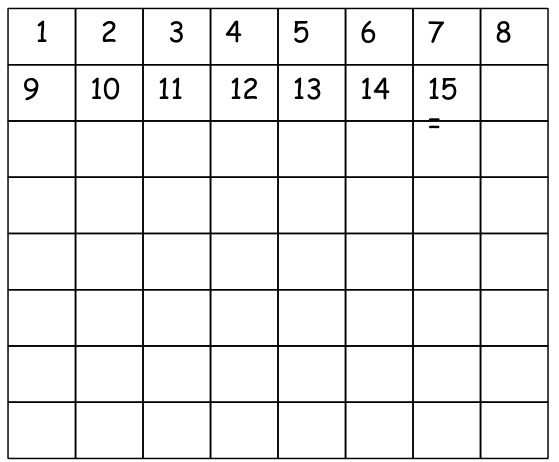
\includegraphics[width=61.11mm,height=127.12mm]{../../images/llm/page_053_img_01.png}%
\end{textblock*}

\end{document}
